\documentclass[final,letterpaper]{article}

\usepackage{url}
\usepackage{graphicx}
\usepackage{hyperref}
\usepackage{pdfpages}
\usepackage{geometry}

\newcommand{\baposter}{\texttt{baposter}}

\title{The baposter latex poster style}
\author{Brian Amberg and Reinhold Kainhofer}
\begin{document}
\maketitle
\begin{abstract}
This is still only a very rough documentation, but it should be better than no
documentation. If anything is unclear, please post a request (preferably with a
patch) at the bugtracker.
\end{abstract}

\section{Introduction}
\baposter{} is a LaTeX template to efficently design pretty posters for
scientific conferences. Posters are composited of blocks with headings, which
can be positioned easily on the page, using absolute or relative positioning. A
number of predefined styles can be composed to generate new color schemes and
ornaments.

\section{Usage}
Refer to the included example posters for the overall structure. I will document the different keys here.
The main environment for the poster is the \texttt{poster} environment. It has the following structure
\begin{verbatim}
\begin{poster}{
  key=value options
  }
  {
    Eye Catcher, empty if option eyecatcher=no
  }
  {
    Poster Title
  }
  {
    Poster Authors
  }
  {
    University Logo
  }

  Definition of the boxes

\end{poster}
\end{verbatim}
\begin{center}
  \setlength{\fboxsep}{0pt}
  \fbox{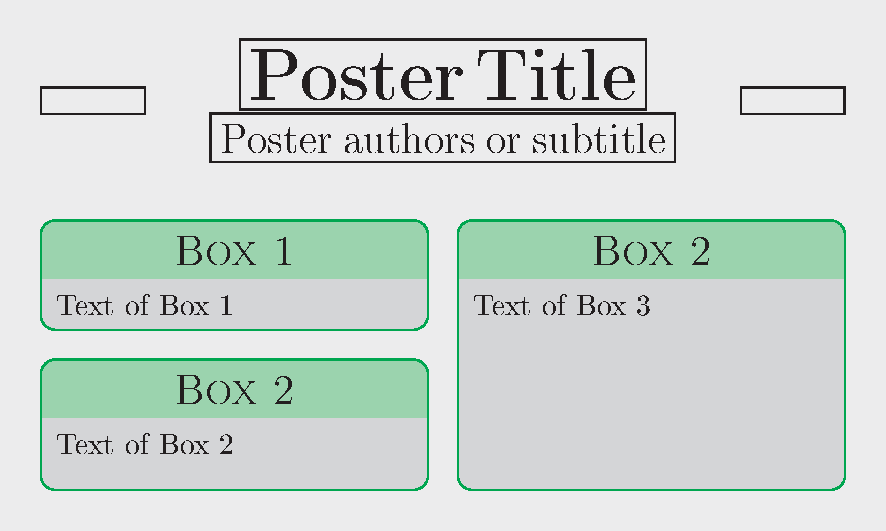
\includegraphics[width=0.9\textwidth]{docs-structure}}
\end{center}

It should be immediately inside the
\begin{verbatim}
\begin{document}
\end{document}
\end{verbatim}
environment, or there will be blank pages.

Additionally, you can pass some options for page size selection directly to the class file.
\begin{verbatim}
\documentclass[class options]{baposter}
\end{verbatim}

\subsection{Class Options}
The class options are

\begin{description}
\item [landscape/portrait] Page Layout
\item [a0paper, a1paper, a2paper, a3paper, a4paper, archE] Predefined paper sizes
\item [paperwidth=length,paperheight=length] Width/Height of the paper. Do not use together with a0paper or other predefined paper sizes.
\item [margin=length] Page margin
\item [fontscale=real number] Scaling of the poster. The poster is typeset with
standard font sizes on a `fontscale times papersize' paper, and then scaled up
by 1/fontscale to the chosen paper size. This ensures good looking font sizes.
So if you need to fit more onto a poster, increase the fontscale option to get
smaller fonts. But be sure not to choose too small fonts, or your paper will be
awful. I find posters with small print a nuisance, and tend to spend more time
with well presented and concise content.
\item [showframe] Show a frame around the page, mainly useful for debugging.
\end{description}

\subsection{Poster Environment Options}

The available options are:
\begin{description}
  \item[grid=\{yes,no\}]                Display a grid, which can be useful during the layout phase.
  \item[columns=4] Number of columns (default 4 in landscape and 3 in portrait format) (maximum number is 6)
  \item[colspacing=length]              Distance between the columns of the poster
  \item[headerheight=length]            Height of the main poster header as a length (not of the headers of the text boxes). Default value is \verb+0.1\textheight+.
  \item[background=poster background type] Type of poster background. Possible values are
  \begin{enumerate}
    \item \verb+plain+: Plain background in one color (\verb+bgColorOne+)
    \item \verb+shade-lr+: Horizontal background gradient (from \verb+bgColorOne+ to \verb+bgColorTwo+)
    \item \verb+shade-tb+: Vertical background gradient (from \verb+bgColorOne+ to \verb+bgColorTwo+)
    \item \verb+user+: Use the command \verb|\background{...}| to define your own background.
    \item \verb+none+: No background at all.
  \end{enumerate}
  \begin{center}
    \setlength{\fboxsep}{0pt}

    \fbox{
\includegraphics[width=0.21\textwidth,page=1]{docs-background}}
    \fbox{
\includegraphics[width=0.21\textwidth,page=2]{docs-background}}
    \fbox{
\includegraphics[width=0.21\textwidth,page=3]{docs-background}}
    \fbox{
\includegraphics[width=0.21\textwidth,page=4]{docs-background}}
  \end{center}

  \item[bgColorOne=pgf color name]      First background color. For a plain, this color will be used. For a shaded background, this is the first color for the gradient.
  \item[bgColorTwo=pgf color name]      Second background color. This color will only be used for shaded backgrounds as the end color of the gradient.
  \item[eyecatcher=\{yes,no\}]           Should an eye catcher be shown on the
                                         left of the title page. The eyecatcher itself is defined in the second
                                         argument of the poster environment.

\end{description}

\subsection{Posterbox Environment Options}

\begin{description}
  \item[borderColor=pgf color name]     Color used for the borders of the poster boxes
  \item[headerColorOne=pgf color name]  First color of box header. Two colors can be used to define gradients.
  \item[headerColorTwo=pgf color name]  Second color of box header. Two colors can be used to define gradients.
  \item[textborder=border type]         Which kind of border should the lower part of the text boxes have. Possible values are:
  \begin{enumerate}
    \item none
    \item bars
    \item coils
    \item triangles
    \item rectangle
    \item rounded
    \item faded
  \end{enumerate}
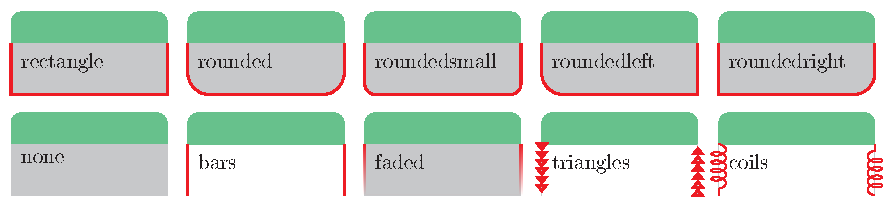
\includegraphics[width=0.9\textwidth]{docs-boxshape}

  \item[headerborder=header border type] At which sides of the text box headers should we draw a border. Possible values are:
  \begin{enumerate}
    \item none
    \item closed
    \item open
  \end{enumerate}

\includegraphics[width=0.9\textwidth]{docs-headerborder}
  \item[headershape=header border shape] The type of ornament of the text box headers. Possible values are
  \begin{enumerate}
    \item rectangle
    \item small-rounded
    \item roundedright
    \item roundedleft
    \item rounded
  \end{enumerate}

\includegraphics[width=0.9\textwidth]{docs-headershape}
  \item[headershade=type of header shading] Which shading should be applied to the text box headers. Possible values are
  \begin{enumerate}
    \item plain
    \item shade-lr
    \item shade-tb
    \item shade-tb-inverse
  \end{enumerate}
  \item[boxshade] which kind of shading is applied to the text boxes. Possible values are
  \begin{enumerate}
    \item shade-lr
    \item shade-tb
    \item plain
    \item none
  \end{enumerate}
  \item[headerfont=font definition]      Commands inserted before a text box header is typeset.
  \item[headerFontColor=pgf color name]  Color that the header is typeset in.
  \item[linewidth=length] Width of the lines used when drawing the poster.
\end{description}

\section{Author and Licence}
The original author is Brian Amberg, and the class and documentation has been
greatly improved by Reinhold Kainhofer. The class is distributed under the GPL.
The current version and documentation can be found at:
\begin{center}
\url{http://www.brian-amberg.de/uni/poster/}
\end{center}
\end{document}

